\documentclass{mpaper}

\begin{document}

\title{Measuring Software Ticket Quality using Quantitative Data Analysis}
\author{Andrei-Mihai Nicolae}
\matricnum{2147392}

\maketitle

\begin{abstract}
Software tickets are of valuable importance to the whole computing science 
field - they guide engineers towards better planning, management 
and tracking of their progress throughout complex projects. However, there
are few studies that investigate what makes for a high quality,
valuable ticket. This can lead to multiple issues in a company, such as 
increased communication friction between developers and end users filing bug
reports, as well as increased overall costs due to waste of development effort. 
In this research paper, we present our findings after 
investigating a large number of variables surrounding software tickets, 
such as whether the presence of stack traces influence the time 
to close for the ticket. Our results show that the presence and type of attachments,
comments complexity (i.e. number of comments per ticket), grammar correctness scores
as well as the sentiment drawn from the comments can influence the quality of the ticket.
We bring a couple of novel aspects to the research
community including one of the largest dataset statistically analysed in the field,
as well as state-of-the-art sentiment and grammar correctness analysis.
\end{abstract}

\section{Introduction}


In the past decade, technology has drastically increased its influence on 
virtually every aspect of our society. Therefore, software projects have 
inherently become more complex and require increasing number of developers in
the team. Due to this, software engineers have created issue tracking systems,
a means of planning, managing and tracking work products in the form of 
\emph{software tickets} or \emph{issues}.

There are multiple platforms for providing such issue tracking systems, among which
the most popular are Jira \cite{jira} and Bugzilla \cite{bugzilla}. For both platforms,
the tickets are split into two main categories: feature requests (i.e. feature to be 
implemented into the system) and bug reports (i.e. issue encountered by an end user or
discovered by a developer in the codebase). Regardless of the type of ticket, they provide
various types of information that can be filled in by the reporter, including:
  \begin{itemize}
    \item summary - short description of the feature to be implemented/encountered bug;
    \item description - longer textual field which goes into more detail regarding the ticket;
    it can include various types of information, such as stack traces or steps to reproduce a bug;
    \item attachments - screenshots, snippets of code or configuration files that might help
    close the ticket faster;
    \item comments - each ticket can have any number of comments where the people interested in 
    it can talk about what might have caused the bug, how to fix it etc.
  \end{itemize}

Even though tickets provide such comprehensive information regarding a specific task, studies have shown 
that fixing bugs is one of the most common tasks performed by developers \cite{latoza2006maintaining}. One of
the reasons for this is the communication friction between developers and end users \cite{Korkala2014WasteIdentification}
as developers might need clarification regarding what information the users have provided (e.g. cannot reproduce the bug, 
screenshot is unclear). Another main reason for this waste of effort on solving tickets, according to 
Just et. al \cite{just2008towards} and Zimmermann et. al \cite{zimmermann2009improving}, is the generally poor design of issue 
tracking systems. This can lead to various issues, including increased costs for the company, wasted development effort, 
decreased customer satisfaction and overall poor performance.

Therefore, there is a need in the community to find the answer to what makes for a high quality, valuable software ticket 
that would improve the overall performance of the development team and, inherently, the company. As there are many 
fields in a ticket, there are numerous unanswered questions: do stack traces have an influence on the quality
of a ticket? What about attachments and whether a screenshot is more helpful than a snippet of code? Does a negative sentiment
drawn from comments increase or decrease the time taken to solve a bug? How does grammar correctness influence the 
communication friction?

In this research paper, we present and discuss our findings after running a quantitative data analysis 
on over 300,000 tickets taken from more than 15 open source projects. We have implemented a Go application 
with multiple commands (i.e. store, analyze, plot, statistics) that can automatically fetch any number of tickets 
from a Jira instance, analyze them, generate plots and run statistical tests. 

During the analysis part, we investigate several variables in correlation with \emph{time-to-complete}, 
which we define as the \emph{metric of quality}. \emph{time-to-complete} represents the period of time between the creation 
and the closing of a ticket; more specifically, the creation of the ticket is marked when the status of the ticket is set to 
\emph{Open} and the closing of a ticket is considered when the ticket status is set to \emph{Closed} (or some similar status, 
such as \emph{Fixed}, \emph{Resolved}). \emph{Time-To-Complete} is our dependent variable, and as independent variables 
(i.e. variables controlled in order to test the effects on the dependent variable) we have set a number of ticket fields. 

This study brings several contributions to the research community:
\begin{itemize}
  \item it is one of the very few research projects that investigates such a large number of tickets (over 300,000) spanning
  across a variety of projects (i.e. 21 projects);
  \item it is one of the few studies in the field that performs a quantitative analysis rather than a qualitative one;
  \item it is, to our knowledge, the first study to conduct sentiment and grammar correctness analyses on software tickets.
\end{itemize}

In Section \ref{related_work} we iterate over state-of-the art studies in the field and then continue with 
Section \ref{building} where we discuss how the ticket data set was collected and analysed. We continue with describing 
the data set (Section \ref{characterising}) where we provide insights into various aspects of the data (e.g. size of database,
number of tickets with attachments) and then discuss about correlations between the variables (Section \ref{correlations}).
Finally, we provide future research directions in Section \ref{future_work} and present our conclusions in Section \ref{conclusions}.

\section{Related Work}\label{related_work}

\begin{figure*}
\begin{center}
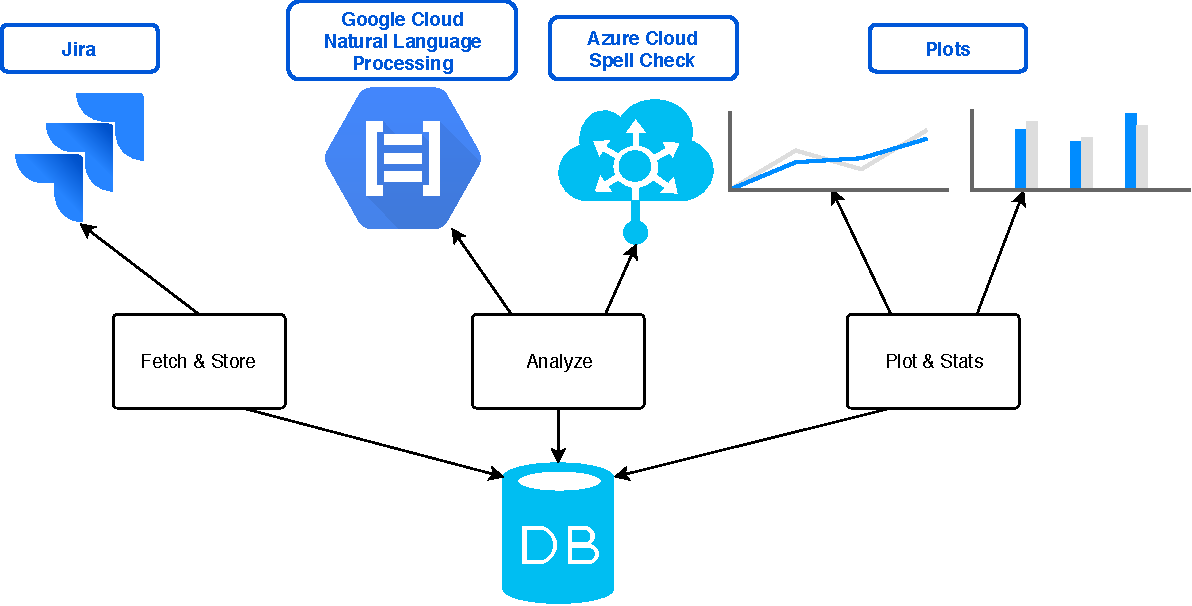
\includegraphics[width=\textwidth]{images/flow.pdf}
\end{center}
\caption{\label{fig-eg}Application flow of the Go tool.}
\end{figure*}


\section{Building the Data Set}\label{building}
The first step towards building the data set was to create a tool that was able to execute all the commands that we required:
fetching the tickets from any Jira instance, storing them into some form of database, analyze the variables of interest, 
automatically plot the correlations between them and run statistical analysis on the data. After careful consideration, 
we decided that Go was the best way to go for various reasons:
  \begin{itemize}
    \item it is designed with simplicity in min, thus making it easier for others who might join the project to read 
    and understand the codebase;
    \item it is compiled, statically typed, which implies that it is a much faster candidate than other interpreted languages
    such as Ruby or Python;
    \item is is designed with concurrency in mind, thus it helps reduce times of execution and computing power considerably;
  \end{itemize}

Then, we split our tool into four main commands: \emph{store}, \emph{analyse}, \emph{plot} and \emph{stats}. They all 
follow the flow shown in figure \ref{fig-eg} and complete the whole application cycle, in the end producing a database 
of analysed tickets, as well as plots and statistics for investigating correlations, saved on the filesystem.

In the following two subsections we describe how we designed and implemented the commands mentioned above.

\subsection{Fetch and Store}

This is the first command implemented in our tool - it is desgined to fetch, from any valid Jira URL, any number of tickets 
and then store everything inside an instance of BoltDB \cite{bolt}, which is a very simple yet powerful key-value pair 
database. The whole process is parallelized with the possibility of scaling even up to hundreds of goroutines
(i.e. lightweight threads) running concurrently.

We have interacted with the Jira Server REST API which has very good documentation written by the Atlassian team. After getting
familiar with all the features the REST API offers, we have opted for getting paginated issues from the server, which means 
slicing the whole set of tickets into multiple smaller arrays to improve performance and reduce the load on the server. We also
specified to Jira exactly what set of issue fields to return and, eventually, while responses were retrieved from the instance,
we began storing them into our Bolt DB instance. The way we chose to store them was to set the issue key (i.e. unique 
identifier that differentiates a ticket from all others across all projects inside a Jira instance) as the key of the pair and
the value is the whole representation of an issue (e.g. attachments, story points, priority) as a JSON encoded value. This
helped us reduce the size of the database once we reached hundreds of thousands of tickets.

\subsection{Analyse}

Once the Bolt DB instance is completely populated with all the tickets we were interested in, the analyze command first 
fetches all the issues in the database. Then, it runs in parallel the \emph{seven types of analysis}:
\begin{itemize}
  \item \emph{attachments} - checks whether attachments influence Time-To-Close and also look at what types 
  of attachments (e.g. screenshots, archive, code snippets) influence quality the most;
  \item \emph{steps to reproduce} - performs a complex regex to detect steps to reproduce and then checks whether their presence
  influence the quality of a ticket;
  \item \emph{stack traces} - runs complex regex for detecting stack traces in either summary, description or comments 
  and verifies whether their presence influence Time-To-Close for the ticket;
  \item \emph{comments complexity} - loops through all comments and counts all words; then, the tool verifies whether 
  having many words or comments decreases or increases Time-To-Close for the ticket;
  \item \emph{fields complexity} - same analysis as comments complexity, but only for summary and description;
  \item \emph{grammar correctness} - it uses Azure Cloud Bing Spell Check API \cite{bing} to perform analysis on summary, 
  description and comments; after concatenating everything and making it compatible with the API allowed formats, the tool 
  receives back in the JSON payload not only the number of flagged tokens (i.e. grammar errors), but also their types 
  (e.g. unknown token, misspell);
  \item \emph{sentiment} - uses Google Cloud Platform's Natural Language Processing API \cite{gcp_nlp} to retrieve the 
  sentiment score for summary, description and comments; it first concatenates everything and makes it conform to Google's 
  API and then sends the request, receiving a score from -1 to 1 inclusive (-1 is completely negative, 1 is completely 
  positive).
\end{itemize}

Implementation wise, the application first checks Bolt for tickets and gets either all of them in memory (easier to parse, 
but heavy on resource utilization) or slices them into smaller arrays to get processed afterwards (harder to parse as it 
eventually requires re-creation of the whole array of tickets before inserting back into the database, but it is much 
lighter on computing power). After having the tickets available, we start looping through them and perform all 
analysis types mentioned above. Once some sort of value is computed (e.g. grammar correctness score), it gets set in 
its corresponding field in the ticket struct and subsequently is stored back in the database. We chose this approach because 
we do not want to run the analysis every time we want to plot correlations between variables, but rather have the data 
already available there. Moreover, for external analysis such as hitting Google Cloud Platform APIs, there are costs for 
running the analysis, thus in this way we drastically reduce overall costs for the project. 

\subsection{Plot and Statistical Tests}

Afterwards, we have created two extra commands for automatically generating plots (i.e. scatter plots and bar charts) and 
running statistical tests on the collected data. 

For plotting the data, we first connect again to the Bolt database instance and then filter out only the issues that have 
the variable \emph{Time-To-Close} set (i.e. tickets marked as closed when they were fetched from the Jira instance). Afterwards,
we either save scatter plots or bar charts to disk. 

Also, in order to validate our findings, the statistics command fetches all the data from the database and 

\section{Characterising the Data Set}\label{characterising}

\section{Correlations}\label{correlations}

\subsection{Attachments}

\subsection{Comments}

\subsection{Summary and Description}

\subsection{Grammar Correctness}

\subsection{Sentiment Analysis}

\subsection{Steps to Reproduce}

\subsection{Stack Traces}

\section{Future Work}\label{future_work}

\section{Conclusions}\label{conclusions}

\vskip8pt \noindent
{\bf Acknowledgments.}
Tim, my parents, Corina.

\bibliographystyle{abbrv}
\bibliography{paper}


\end{document}

% \begin{table}
% \begin{tabular}{l||c||p{2cm}}
% \emph{Operating System} & \emph{Version} & \emph{Verdict} \\ \hline \hline
% Ubuntu & 12.04 & Everyone's favourite Linux, unless you grew up with
% RedHat \\ \hline
% Slackware & xxx & Pseudo-hacker's Linux, how often do you recompile
% your kernel? \\ \hline
% Mac OS & 10.7 & For people with more money than sense \\ \hline
% \end{tabular}
% \caption{\label{tab-eg}Single column table of figures}
% \end{table}

% \begin{figure*}
% \begin{center}
% 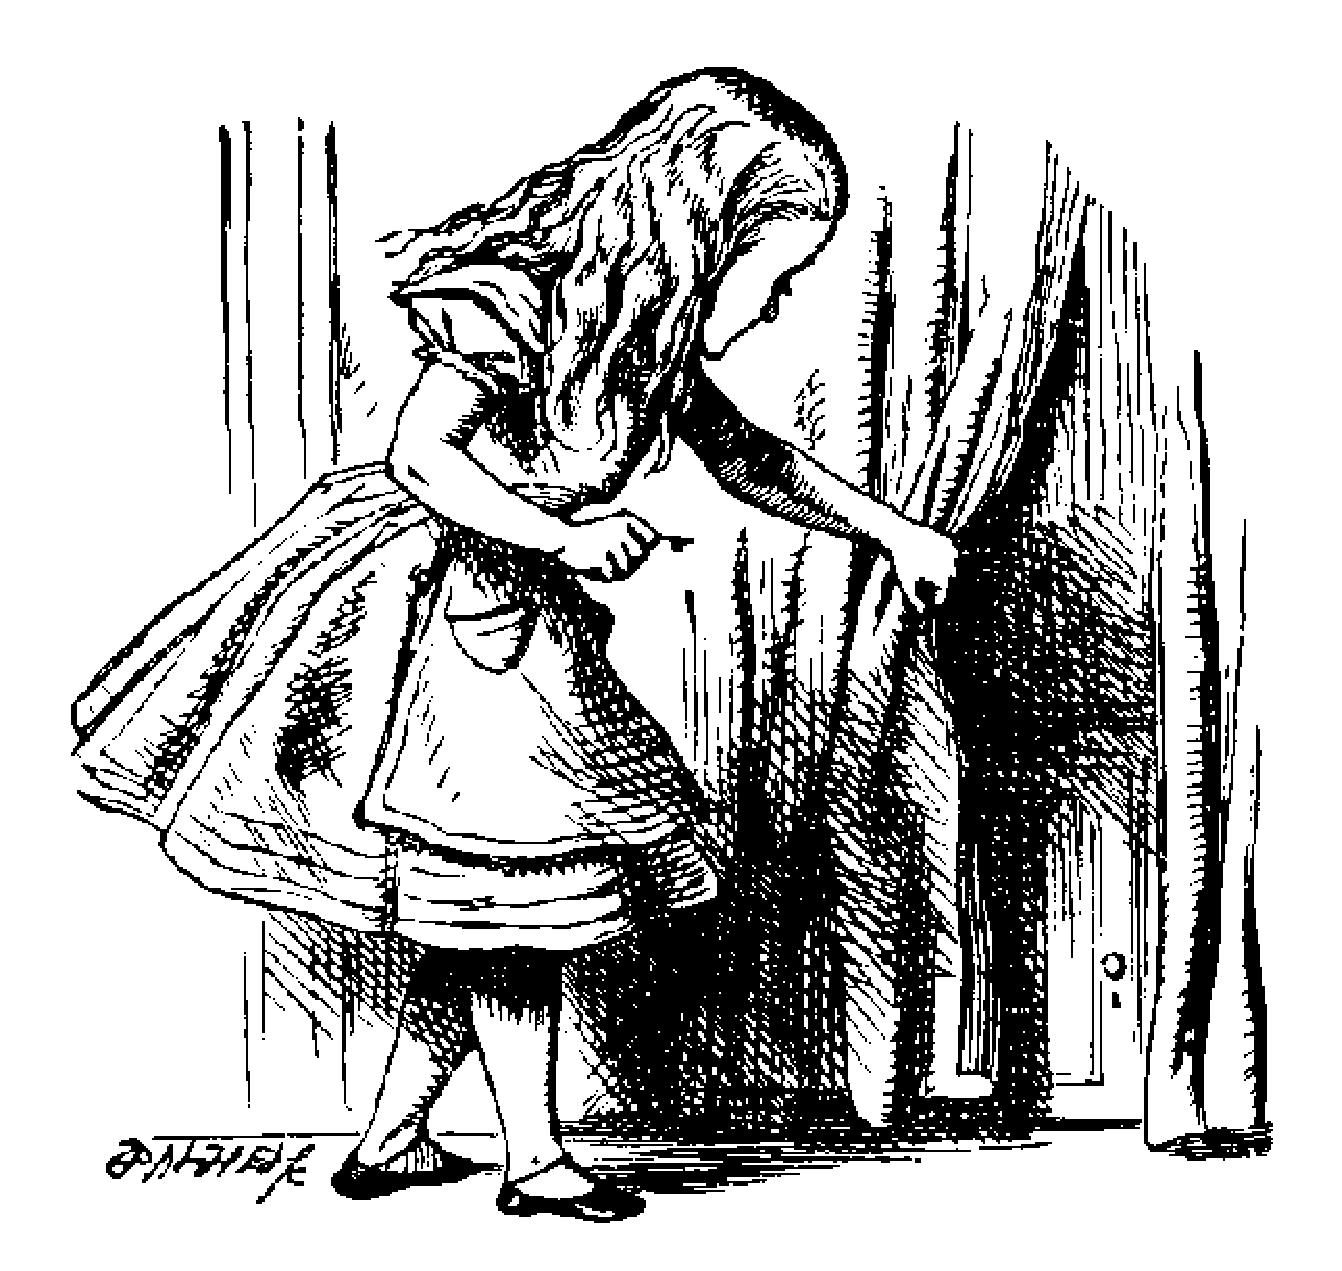
\includegraphics[scale=0.3]{images/alice.pdf}
% \end{center}
% \caption{\label{fig-eg}An example figure stretching over two columns}
% \end{figure*}